\phantomsection
\section*{一、引言}
\addcontentsline{toc}{section}{一、引言}

\phantomsection
\subsection*{1.1 研究背景与应用动机}
\addcontentsline{toc}{subsection}{1.1 研究背景与应用动机}

大语言模型推理的部署正在从云端集中式服务扩展到多个边缘节点参与的协作式服务。现有优化研究主要覆盖两类环境：端侧推理通过模型压缩、量化、小模型和端侧 NPU/GPU 加速，使部分请求能够在用户设备上完成；云端或数据中心推理服务则通过高性能算子、连续批处理、KV Cache 管理、模型并行和多实例调度提高吞吐并降低尾时延。已有系统与综述分别从执行运行时、内存管理、批处理调度和分布式服务等角度总结了这些机制 \cite{yu2022orca,kwon2023efficient,agrawal2024taming,zhong2024distserve,zheng2024sglang}, \cite{zhou2024survey,zhen2025taming,pan2025survey}。

两类环境各有适用边界。端侧推理具有低时延和数据本地性优势，但受算力、内存、功耗和散热限制，难以长期承载复杂大模型和高并发服务。云侧推理资源充足、框架成熟，但网络传输会影响端到端时延、带宽消耗、隐私边界和服务可用性。与此同时，基站、网关、园区和近用户位置已经部署了大量分散、异构且动态变化的边缘算力；这些资源规模大于单个端侧设备，又缺少数据中心同构集群的稳定互联与统一规格。

本文所讨论的 CEC（Collaborative Edge Computing，协作边缘计算）将地理分布、能力异构的终端设备、边缘服务器和 AI 板卡组织为协作资源池，并借助 Wi-Fi 接入点、路侧单元、5G 基站和网关等基础设施交换请求、中间结果与运行时状态。如图~\ref{fig:collaborative-edge-computing} 所示，多个边缘资源可以共同完成模型部署和推理执行，请求路径不依赖预设的端、边、云三级结构。终端可以作为请求入口或计算节点，CEC 不是为了替代中心化的云，而是作为补充，外部云服务则在业务允许时作为可选服务或异常回退路径。分布式协同智能研究为异构资源、链路和服务位置的联合优化提供了参考 \cite{duan2022distributed}；本文聚焦协作边缘资源池内部的模型切分、请求调度和状态管理。相应的系统问题是：如何在资源与网络持续变化的条件下，以可控成本满足业务时延、吞吐、服务连续性和数据隐私要求。

\begin{figure}[htbp]
    \centering
    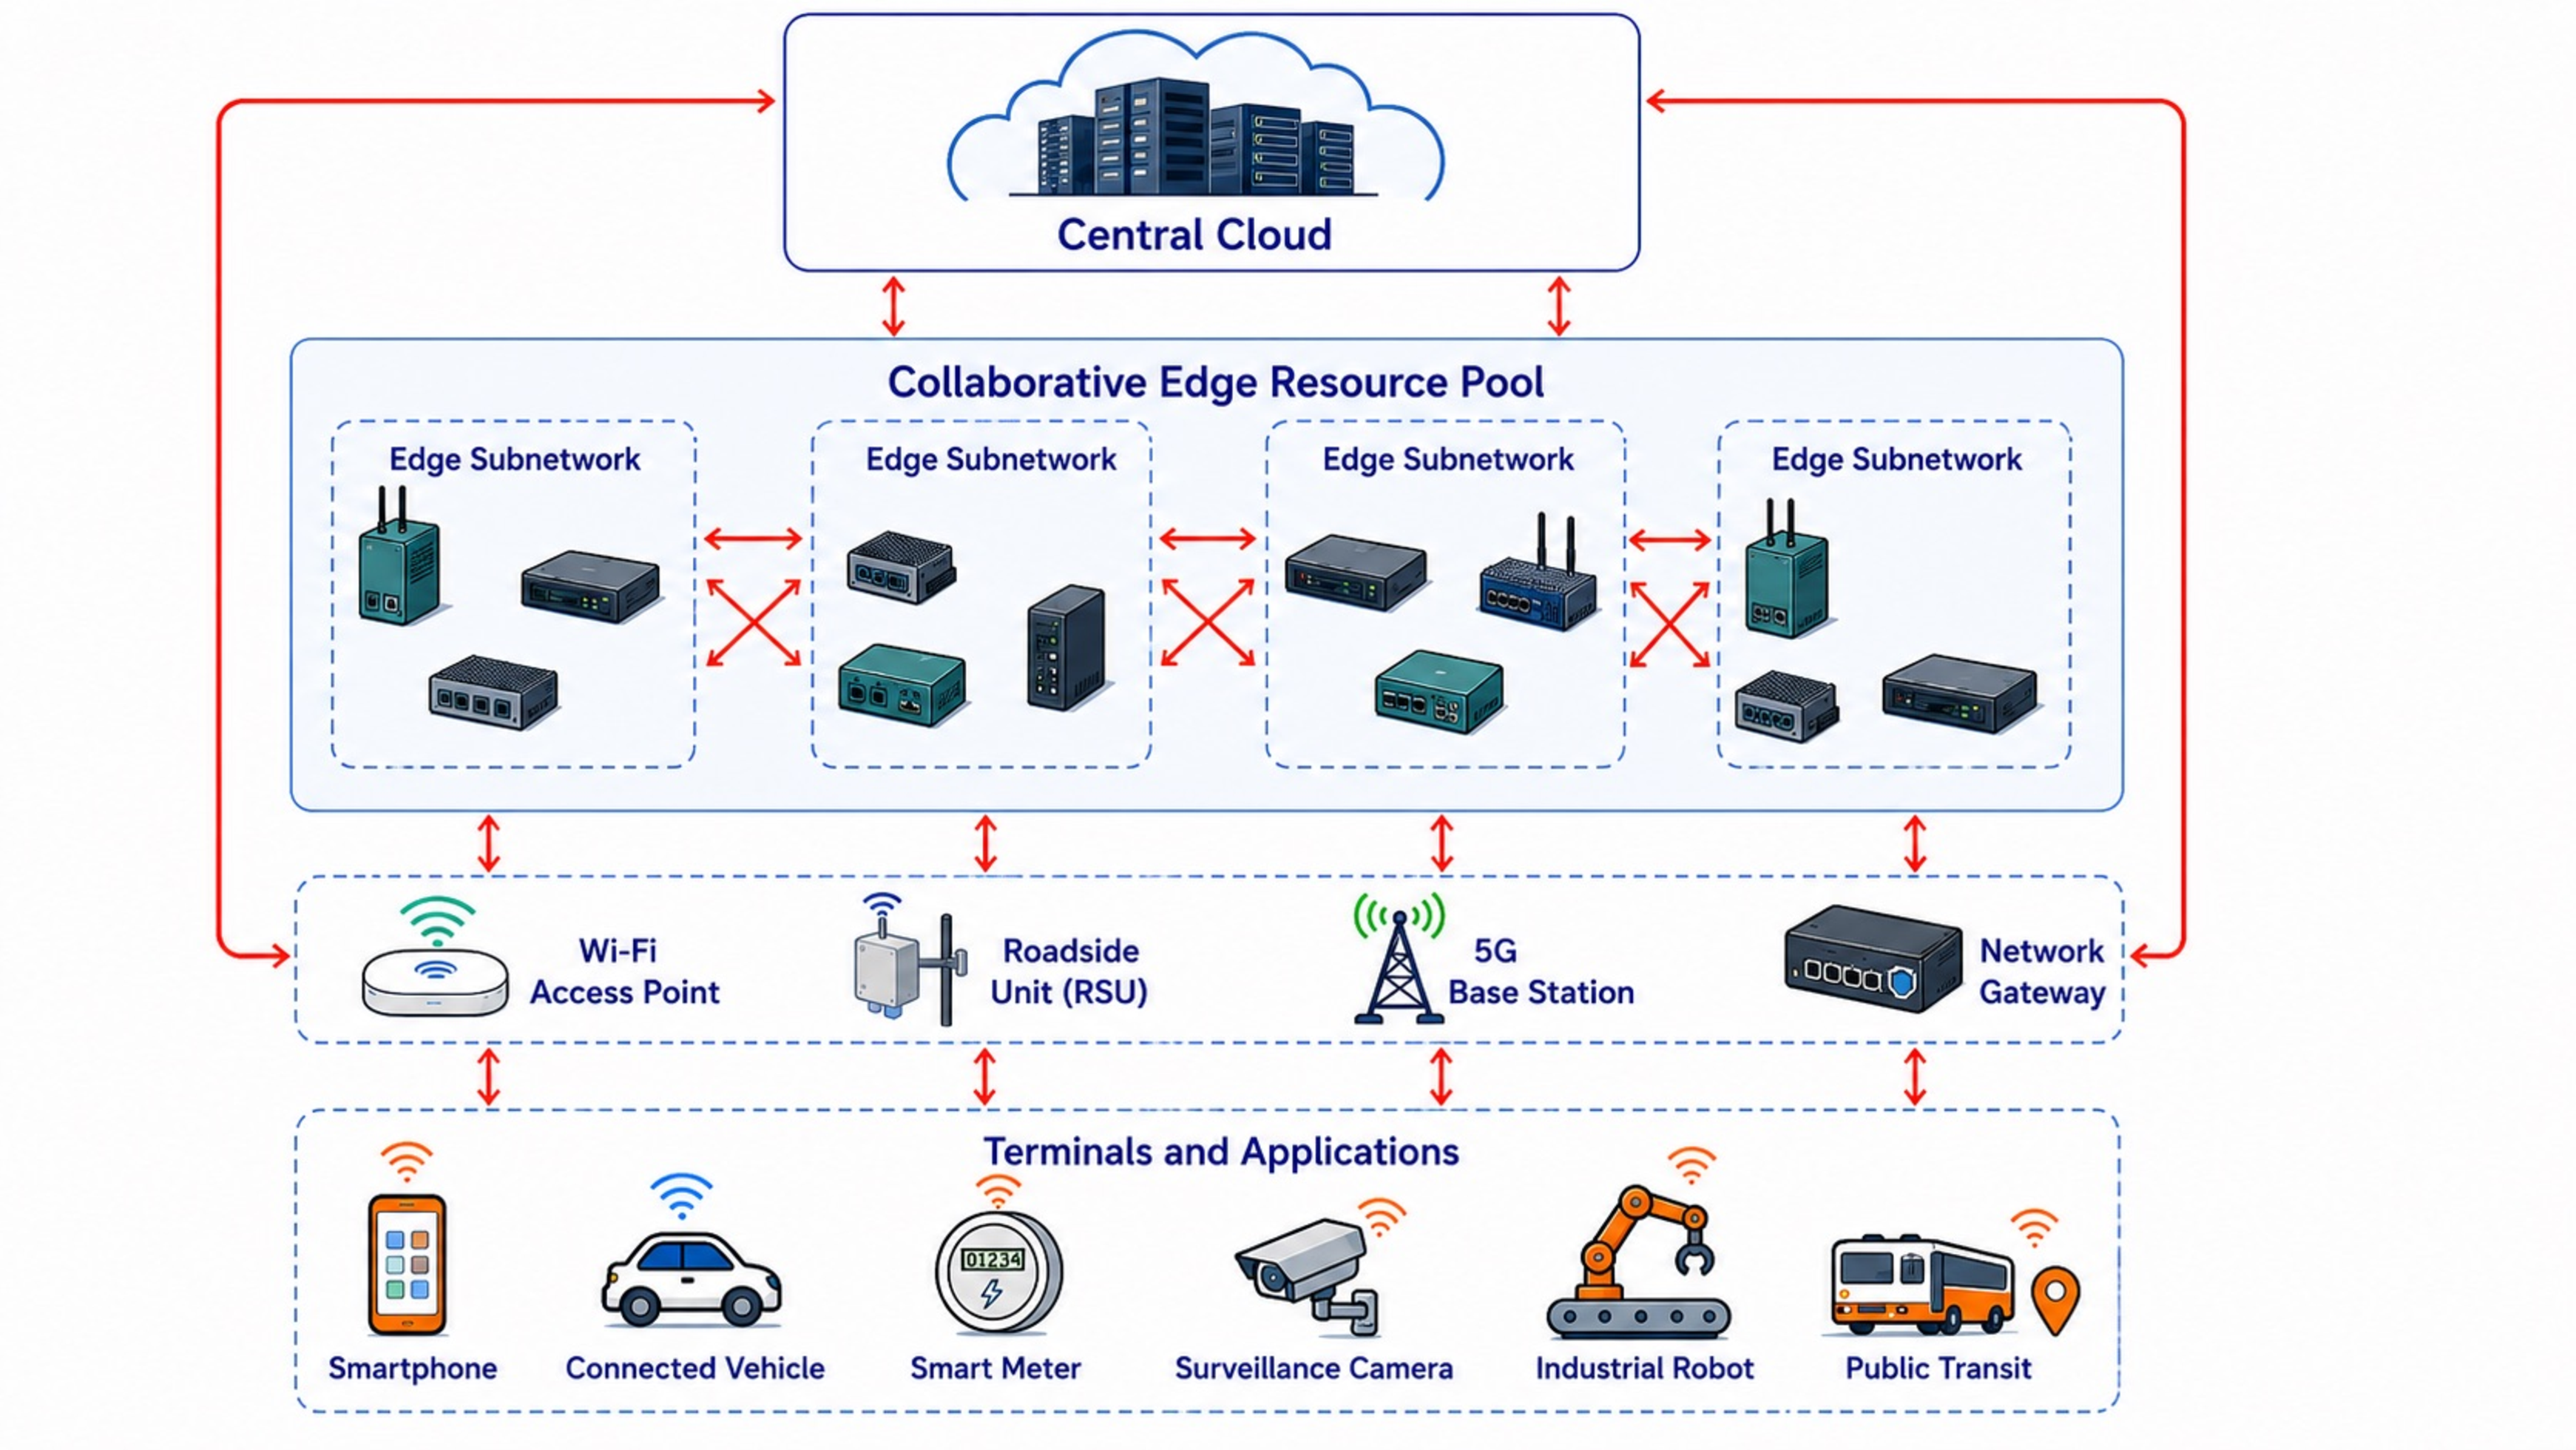
\includegraphics[width=\textwidth]{figures/ch1_collaborative_edge_computing.pdf}
    \caption{\textbf{协作边缘计算示意图。}协作边缘计算汇聚泛在、地理分布设备的计算资源以共同执行计算任务，从而扩展可用资源池，实现低时延数据处理、灵活设备接入与更广的服务覆盖。}
    \label{fig:collaborative-edge-computing}
\end{figure}



\phantomsection
\subsection*{1.2 CEC 场景下边缘 LLM 推理的关键挑战}
\addcontentsline{toc}{subsection}{1.2 CEC 场景下边缘 AI 推理的关键挑战}
然而，CEC场景给 LLM 推理带来了新的挑战，具体如下

\textbf{CEC 场景下的边缘 AI 推理首先受到资源异构和碎片化的约束。}终端设备以及部署在基站、网关、园区和边缘服务器中的 GPU、NPU 与 AI 板卡，在算力、内存、显存、功耗预算和加速库支持上差异显著，模型部署不能直接套用数据中心中“节点规格相近、互联稳定、控制面统一”的假设。同一个模型在不同硬件上可能面临完全不同的显存瓶颈、算子支持和通信代价，部署策略也必须随资源状态动态调整。

\textbf{LLM 推理本身还具有显著的状态和内存压力。}Prefill 阶段会为后续 decode 生成 KV Cache，decode 阶段又会随着输出长度不断追加状态；在长上下文、多轮会话和高并发场景中，KV Cache、prefix cache 和 session state 会长期占用显存，并要求系统管理其生命周期、位置和一致性。一旦这些状态跨节点访问、迁移或重算，通信成本、服务连续性和隐私边界都会同时受到影响。

\textbf{请求动态性进一步放大了调度难度。}用户并发数、prompt 长度、输出长度、请求复杂度和时延 SLO 都在持续变化，边缘节点又常常缺乏云侧的大规模请求池，静态 batching、固定 batch size 和固定服务路径难以稳定满足业务要求。对于移动用户，接入点和合适的服务实例还会随位置变化；距离最近的节点未必具有最短的排队时间或端到端时延。若用户会话中的 KV 或上下文状态仍保留在原服务节点，服务切换还可能引发状态迁移、远程访问或重新 prefill。

这些因素相互影响：模型切分会改变各节点的计算量和跨节点 activation 传输，batching 会改变排队时间、KV 占用和设备利用率，请求卸载又会改变流量分布与状态位置。因而，CEC LLM inference 需要联合比较计算收益、通信开销和状态迁移成本，并在业务时延、隐私和服务连续性约束下选择可执行的部署与调度方案。


\phantomsection
\subsection*{1.3 相关研究基础与问题主线}
\addcontentsline{toc}{subsection}{1.3 相关研究基础与问题主线}

现有研究为 CEC LLM inference 提供了多方面基础。一方面，on-device inference 关注模型压缩、低比特执行、小模型设计和端侧硬件加速，使部分请求能够在用户设备本地完成；FlexGen~\cite{sheng2023flexgen}、Petals~\cite{borzunov2023petals}、HexGen~\cite{jiang2023hexgen} 等工作则进一步展示了资源受限或异构环境下的大模型推理可以通过分层存储、协作式 block 放置和异构并行来突破单节点容量限制。另一方面，cloud/datacenter LLM serving 已经围绕 continuous batching、PagedAttention、chunked prefill、prefill/decode disaggregation、KV cache management 和多实例调度形成了较成熟的系统路线，Orca~\cite{yu2022orca}、vLLM~\cite{kwon2023efficient}、Sarathi-Serve~\cite{agrawal2024taming}、DistServe~\cite{zhong2024distserve}、SGLang~\cite{zheng2024sglang} 和 Mooncake~\cite{qin2025mooncake} 等系统分别代表了不同层面的关键机制。

边缘计算领域长期研究任务卸载、资源分配、移动性管理和网络感知调度，其中许多卸载模型将任务描述为具有固定输入大小、计算量、deadline 和能耗约束的作业。LLM 推理的服务时间还取决于 prompt、输出长度、decode 进度、batch 组成和 KV 状态，复杂请求也可能涉及多模型、多智能体或多阶段执行。因此，CEC LLM 推理同时包含 LLM serving 中的 prefill/decode、KV Cache、batching、推测解码和分布式执行问题，以及协作边缘环境中的资源异构、动态网络、用户移动、隐私约束和服务连续性问题。

基于这一交叉特征，本文将相关工作组织为三条主线。第一条是 \textbf{CEC 下的资源自适应模型部署方法}，关注模型结构、模型组件和推理阶段如何在异构协作节点之间切分与放置。第四章的综述覆盖 layer、tensor、expert、推理阶段和生成职责等不同切分对象，面向验证环境的具体方案则先比较 TP、PP 和 PP+TP，再采用动态规划求解非均匀 PP 的连续 layer 分割。第二条是 \textbf{CEC 中的业务感知 batching 参数优化算法}，关注请求进入推理实例后如何根据 SLO、队列状态、KV 占用和 prefill/decode 干扰选择 batch 形成与更新策略，具体方案采用 Safe-RL 联合调节 batch 参数、请求顺序和运行时机制。第三条是 \textbf{CEC 中的 LLM inference task offloading}，关注完整请求、会话、multi-agent workflow 以及 context/KV/runtime state 如何在协作边缘节点之间路由、卸载、迁移和复用。这三条主线分别对应模型部署、实例内调度和跨节点服务路径选择。


\phantomsection
\subsection*{1.4 研究范围与内容组织}
\addcontentsline{toc}{subsection}{1.4 研究范围与内容组织}

本文聚焦 \textbf{CEC 场景下的大语言模型推理优化问题}。研究范围限定在推理阶段，不讨论大模型训练、预训练或微调过程；重点关注终端设备、边缘服务器、AI 板卡以及部署在基站、网关和园区中的推理节点之间的大模型推理协同，包括资源自适应模型切分与部署、动态 batching、prefill/decode 调度、分布式 KV/状态管理、任务卸载、请求路由、移动性感知调度和服务连续性保障。


底层算子优化、硬件实现和模型结构设计仅在影响 CEC 推理系统时纳入讨论。例如，低比特算子会影响模型能否部署到目标设备，KV Cache 布局会影响状态迁移和缓存复用，便于切分的模型结构会影响跨异构节点执行的可行性。本文从系统角度分析这些因素对部署、调度、状态管理和服务策略的影响。

本文首先从 prefill/decode、KV Cache、batching/scheduling、decoding runtime 和主要服务指标出发，梳理 LLM inference 的基本执行机制，并解释模型规模、KV 状态、请求动态性、decode 串行性和多实例协同带来的系统瓶颈。在此基础上，本文构建“优化对象--执行范围”二维分类，将方法按主要优化对象划分为 Model、Kernel、Runtime 和 Serving Policy \& Routing 四层，并区分单实例或本地控制域内的优化与跨设备、跨节点的分布式优化。

随后，本文分析 CEC 环境如何改变 LLM inference 的部署与调度条件，并围绕资源自适应模型部署、业务感知 batching 和 LLM inference task offloading 三条主线梳理代表工作。在相关工作分析之后，第四章给出基于动态规划的非均匀 PP 方案，第五章给出基于 CMDP 的 Safe-RL batching 方案，第六章给出联合选择执行节点与 KV 获取方式的长期会话感知卸载方案。第七至第十章进一步讨论三类算法的协同关系、Ascend/vLLM-ascend 实现路线、实验设计及后续研究问题。
